% v1.2, 2026-10-21: corrected-implementation follow-up to the knockout and
% forcing results of v1.0-v1.1, which are WITHDRAWN (the August hooks edited
% the router's returned logits while dispatch used the unchanged ids/weights;
% found by a 2026-09-04 code review, reproduced 2026-10-07). Replaced by a
% dispatch-level rerun on Qwen3.6-35B-A3B (MLX, 4-bit weights, 8-bit router
% gates; 2026-10-07). Layer 26 identified as layer 14's trained copy
% (repeated-block scan v0.1.2, 10.5281/zenodo.23546828); E114 described as one
% of several genre-selective experts (2026-10-01 control); companion record
% re-opened with a status note. All other reported values unchanged from v1.1.
% v1.1, 2026-08-18: single-thesis revision for research-sample use.
% Governing claim carried abstract -> conclusion: in-context availability
% of the target reorganizes expert routing at fixed token identity, is
% carried by attention retrieval, replicates across a model generation,
% and is behaviorally inert at its layer; therefore it is a
% measurement-side confound for multi-turn internal-state evaluations.
% Results reorganized by claim component (not by capture chronology);
% mechanism/replication/intervention compressed to one section plus a
% summary table; informal shorthand ("frozen", "coalition", "carrier",
% "risers", "occupancy", "Task 49", "F01/F02") replaced by standard
% terms; all reported values unchanged from v1.0.2 (verified against
% run logs 2026-08-12), except the exploratory direction-probe component
% averages (-8.8/-7.4), which remain in the artifact release only.
% Earlier history: v0.9 2026-08-11; v1.0 2026-08-12 (cross-generation
% study, mechanism section, interventions); v1.0.2 2026-08-17
% (evaluation-contamination paragraphs). Full log in the .bak files.
\documentclass[10pt,a4paper,twocolumn]{article}

\usepackage[margin=1.75cm]{geometry}
\usepackage[T1]{fontenc}
\usepackage{lmodern}
\usepackage{booktabs}
\usepackage{tabularx}
\usepackage{array}
\usepackage{enumitem}
\usepackage{amsmath}
\usepackage{amssymb}
\usepackage{graphicx}
\usepackage{hyperref}
\usepackage{url}
\usepackage{xcolor}
\IfFileExists{microtype.sty}{\usepackage{microtype}}{}
\IfFileExists{caption.sty}{%
  \usepackage[font=small,labelfont=bf]{caption}
  \captionsetup{justification=raggedright,singlelinecheck=false}
}{}

\graphicspath{{figs/}{./}}

\hypersetup{
  colorlinks=true,
  linkcolor=blue,
  citecolor=blue,
  urlcolor=blue,
  pdftitle={In-Context Availability Reorganizes Expert Routing: A Measurement Confound for Multi-Turn Evaluations of Mixture-of-Experts Language Models},
  pdfauthor={Jeffrey William Shorthill},
  pdfkeywords={mixture-of-experts, expert routing, mechanistic interpretability, in-context availability, evaluation confound, attention retrieval, pre-registration, teacher forcing}
}

\setlength{\columnsep}{0.65cm}
\setlength{\parindent}{1em}
\renewcommand{\arraystretch}{1.08}
\setcounter{dbltopnumber}{2}
\renewcommand{\dbltopfraction}{0.95}
\renewcommand{\textfraction}{0.05}
\newcolumntype{Y}{>{\raggedright\arraybackslash}X}

\newcommand{\Top}{\operatorname{Top8}}

\title{\textbf{In-Context Availability Reorganizes Expert Routing: A Measurement Confound for Multi-Turn Evaluations of Mixture-of-Experts Language Models}}
\author{Jeffrey William Shorthill\\
\small independent researcher \quad \texttt{jws299792@icloud.com}}
\date{\small Version 1.2, October 2026. Preprint; not peer reviewed. License: CC BY 4.0.\\
\small DOI: \url{https://doi.org/10.5281/zenodo.21892999} (resolves to the latest version)\\
\small Companion technical report (program record, re-opened 2026-10-21 with a status note): \url{https://doi.org/10.5281/zenodo.20709736}}

\begin{document}
\maketitle

\begin{abstract}
In a sparse mixture-of-experts (MoE) language model the router selects a
small subset of experts for every token, and that selection is increasingly
read as an internal-state measurement: to characterize specialization, to
audit safety-relevant behavior, and to track reasoning state. We show that
one property of the preceding context, whether the text being processed is
already present verbatim in an earlier turn (in-context availability),
reorganizes routing at scale at fixed token identity and fixed final
prompt. In Qwen3.5-35B-A3B-Base, teacher-forced
response pairs differing only in the prior turn shifted layer-14 selection of
pre-specified register-specific expert sets by \(-0.175\) (95\% prompt-cluster
bootstrap confidence interval \([-0.184,-0.166]\)) and raised a pre-specified
cross-register set by \(+0.058\) (\([0.055,0.061]\)), under expert sets,
estimands, and decision rules fixed before capture. A \(2\times2\) factorial
attributes the shift to literal availability of the target, with prompt
repetition contributing under one tenth, and the shift survives matching on predictive entropy and target surprisal. Attention
retrieval of the prior copy carries about half of it: under availability
roughly half of each target token's attention mass lands on the prior copy,
and masking that attention moves layer-14 routing more than half of the way
back to its no-availability configuration (12 of 12 pairs). The set structure
replicates on instruction-tuned Qwen3.6-35B-A3B under seven expert-level
predictions fixed before capture (7 of 7 confirmed). Versions 1.0 and 1.1 of
this paper reported that excluding or forcing the confirmed experts at layer
14 left generation token-identical; that result is withdrawn here, because
the intervention code edited router logits that the model did not dispatch
on. In a corrected-implementation follow-up (Qwen3.6-35B-A3B on an MLX
build, dispatch verified, 12 prompts, greedy), excluding the four
increase-experts changed the generated text in seven of twelve prompts
without a detected average change in overlap with the available prior
answer, and forcing one increase-expert raised that overlap and changed
eleven of twelve outputs. Layer 26 of this checkpoint is a trained copy of
layer 14, so the earlier layer-26 corroboration is the same signature seen
through a copy; intervening at both copies did not increase the number of
divergent outputs over layer 14 alone. The consequence is methodological: internal-state
measurements taken on multi-turn probes that place later target text in
earlier context partly measure availability in addition to the capability
under test, and replicated observational routing signatures do not by themselves
license causal claims about the experts involved.
\end{abstract}

\section{Introduction}

Expert routing in sparse MoE models is now used as an observable in its own
right. Routing paths are read for linguistic and semantic structure
\cite{antoine2025,olson2025}, for the presence of domain-specialized experts
\cite{wang2026dbes,wang2026}, for reasoning state at fixed emitted tokens
\cite{chen2026}, for context-faithfulness \cite{bai2025}, and as telemetry
for safety auditing \cite{lv2026}. Every such use assumes that the routing
statistic reflects the property under study rather than an incidental
property of the probe. This paper isolates one incidental property that
multi-turn probes routinely vary and that reorganizes routing at scale: the
literal availability, in an earlier turn, of the text the model is currently
processing.

The question is exact. Hold the final user prompt and every scored response
token fixed, and vary only whether the preceding turn already contains that
response verbatim. Does routing change in a direction that can be specified
before the data are collected? If it does, is the change driven by
availability of the response, by repetition of the prompt, or by the greater
predictability of text that is already in context? Is it carried by an
identifiable pathway, does it reproduce beyond the checkpoint on which it was
discovered, and does it matter for what the model generates?

We answer with a study on Qwen3.5-35B-A3B-Base whose expert sets, estimands,
and decision rules were fixed and hash-committed before capture, and three
follow-ups on the same and a successor checkpoint. The central result is:

\begin{quote}
\textbf{At fixed final prompt and fixed target token identities, verbatim
availability of the target in the prior turn redistributes layer-14 top-8
routing in a pre-specified direction: register-specific expert sets fall
steeply while a small cross-register set rises (120 prompts, six output
registers, with and without prompt repetition, surviving matching on
predictive entropy and target surprisal); we call this signed pattern the
routing signature. Attention retrieval of the prior
copy carries about half of the shift; the set structure reproduces on
instruction-tuned Qwen3.6-35B-A3B under predictions fixed before capture;
and, in a corrected-implementation follow-up on that successor checkpoint,
excluding the confirmed increase-experts changes generated text in seven of
twelve prompts without a detected average reduction in overlap with the
available answer, while
forcing one of them increases reuse. The signature is a reliable correlate
of the availability condition; its experts carry a measurable behavioral
load where we intervened.}
\end{quote}

The implication follows directly. Any evaluation that reads internal state
(routing statistics, expert-selection profiles, or classifiers built on
them) from multi-turn probes that repeat or nearly repeat earlier material
is measuring, in part, whether the target text was available for reuse. The
contamination claim is measurement-side: the corrected interventions change
generated text in most prompts with no detected average reduction in reuse
of the available answer, so we make no claim that availability shifts output-level
scores. A second, narrower implication concerns interpretation: an expert
set can pass a pre-specified confirmation with every interval excluding
zero, and the existence and direction of its behavioral load remain a
separate question that only a correctly implemented intervention can
answer. Versions 1.0 and 1.1 of this paper answered it wrongly;
Section~\ref{sec:intervention} says how, and what the corrected answer is.

Design discipline carries most of the evidential weight. Expert sets, the
primary layer, estimands, bootstrap procedure, and pass/fail rules of the main
study were fixed and hash-committed before the confirmatory captures; the
mechanism study, the cross-generation confirmation, and the interventions each
declared their endpoints or predictions before their runs (the corrected
intervention follow-up recorded its predictions in the run script, without
an independently timestamped snapshot). The claims are
correspondingly scoped: the main result is layer-scoped; the histories are
register-matched but not length- or semantics-matched; predictability matching
conditions on post-treatment measurements and so does not estimate mediation;
and the corrected interventions were run on the successor checkpoint at
reduced precision, so they are a follow-up rather than a checkpoint- and
precision-matched replication.

\section{Background and Related Work}

\paragraph{Routing as an observable.}
Sparse MoE layers route each token to a small subset of feed-forward experts
\cite{shazeer2017,fedus2022}. Qwen3.5-35B-A3B has 40 routed text layers, 256
routed experts per layer, top-8 selection (the eight experts with the highest
router logits are active), and an always-on shared expert that bypasses the
competitive router \cite{qwen2026}. Routing is known to depend on more than
token identity: it carries part-of-speech information \cite{antoine2025},
responds to word sense and substitution in large MoEs \cite{olson2025}, and
shows context sensitivity in similarity-annotated text pairs \cite{arnold2024}.
Most directly, Chen et al.\ hold emitted anchor tokens fixed and show that
routing still separates task context, trajectory history, and reasoning-effort
mode \cite{chen2026}; counterfactual analyses probe alternative expert choices
for the same tokens \cite{yoon2026}; and the routed hidden state has been
decomposed into a control signal driving expert selection and an orthogonal
content channel \cite{ye2026}. We do not claim priority for same-token context
sensitivity. We isolate one contextual variable, verbatim availability of the
target, fix a signed group-level prediction before capture, and test it across
six output registers, then ask what the resulting signature does and does not
license.

\paragraph{Expert groups and specialization.}
Router Lens identifies experts associated with context-faithful behavior and
tests their relevance by masking them \cite{bai2025}. How specialized
individual experts are remains contested: a domain-invariant standing
committee of experts has been reported \cite{wang2026}, much routing structure
has been attributed to representation geometry \cite{wang2026myth}, a
pre-registered causal test found apparent modularity largely dissolving under
intervention \cite{salomone2026}, and benchmark work still reports
domain-partitioned activation in the Qwen family \cite{wang2026dbes}. These
results motivate group-level readouts with fixed membership, which is the form
our expert sets take.

\paragraph{Copying and repetition.}
Induction heads provide an attention-side account of in-context copying
\cite{olsson2022}; deterministic decoding can also produce repetition loops
\cite{holtzman2020,welleck2020}, and repetition effects depend on position
\cite{wang2026rep}. Our main design measures exact prior-turn recurrence
behaviorally; Section~\ref{sec:mechanism} measures its attention-side source
directly and intervenes on it, connecting the induction-head account to a
routed feed-forward consequence within one study.

\section{Methods}\label{sec:methods}

\subsection{Model and routing capture}

The subject is \texttt{Qwen/Qwen3.5-35B-A3B-Base}, evaluated on text only. Its
text backbone is a 40-layer hybrid stack laid out as ten repetitions of three
gated-DeltaNet linear-attention blocks followed by one gated softmax-attention
block; every layer contains 256 routed experts, eight of which are selected
per token, plus one shared expert \cite{qwen2026}. We used a byte-pinned
bfloat16 (BF16) checkpoint in the GGUF serialization used by llama.cpp
(SHA-256 \texttt{ec55dfc4ba300b6c...e415}; llama.cpp commit
\texttt{1772701f99dd3fc13f5783b282c2361eda8ca47c}). A custom capture binary
recorded dense router logits at layers 13, 14, 15, and 26; layer 14 was the
pre-specified primary readout and the others were sensitivity analyses. Layer
numbers are zero-indexed. For every token the top eight experts are
reconstructed by ranking the 256 router logits; all results use top-8
membership, and the shared expert is excluded from every metric. Generated
dialogue used temperature 0.7 (\texttt{top-k 0}, \texttt{top-p 1.0},
\texttt{min-p 0.0}), three seeds, a 180-token response cap, and a 4,096-token
context.

\subsection{Pre-specified prompt bank and expert sets}

The primary bank contains 120 prompts: 20 each in reflective first-person
(REG), technical (TECH), legal (LEGAL), narrative (NARR), poetic (POET), and
code (CODE) registers. A third-party language model generated 30 prompts per
register; within each register, prompts were sorted by ascending SHA-256 of a
salted tuple (salt \texttt{task49-powered-v1-20260709}, register, probe ID,
prompt text), the first 20 hashes formed the primary bank and the remaining 10
an unused holdout. Neither model output nor routing was consulted, and the
bank, split, and validation rules were fixed before capture.

Two kinds of expert set were fixed before the present bank was captured, from
earlier discovery data on the same checkpoint. The layer-14 cross-register set
\(C=\{78,127,143,151,208,210,217\}\) is the intersection of experts whose
selection rose in at least five of six registers across each of three prior
temperature-0.7 discovery seeds. Each register \(r\) has a separate ten-expert
register-specific set \(P_r\), defined from own-register versus other-register
selection on fresh first-turn responses in the discovery data. The discovery
analysis labelled these sets by the contrasts that produced them; the labels
attribute no function, monosemanticity, necessity, or causal role to any
expert, and we use only the neutral symbols \(C\) and \(P_r\) here. No
exploratory expert could replace a member or rescue a failed endpoint. Full
identities and provenance are in the artifact release.

\subsection{Three history designs}

All designs compare a target response processed with and without a preceding
turn that already contains it. We refer to the final user prompt together with
the scored response as the \emph{endpoint}. In the teacher-forced designs the
target response tokens are supplied as input and scored rather than generated,
so token identities are identical across conditions by construction.

\paragraph{Generated repeat-versus-varied study.}
For each target prompt \(p\), register, and seed, the \emph{repeat} arm asks
\(p\) on turns 1, 2, and 3; the \emph{varied} arm asks two deterministic
same-register prompts (at within-register offsets \(i+7\) and \(i+13\) modulo
20 for target index \(i\)) on turns 1 and 2, then asks \(p\) on turn 3. Turn-3
prompt, dialogue position, register, and seed are matched; the histories
differ jointly in prompt repetition, prior-answer availability, and whole-turn
matching. This yields 2,160 responses and 360 paired turn-3 endpoints. For each
generated token we find the longest suffix \(n\)-gram ending at that token
that occurs in an earlier assistant turn; the \emph{copy fraction} of a
response is the share of its tokens whose longest match is at least eight
tokens. The pre-specified manipulation check required a repeat-arm median copy
fraction of at least 0.50, a median paired difference of at least 0.30, and at
least 70\% of repeat endpoints at or above 0.50.

\paragraph{Matched-token study.}
Its analysis plan was hash-committed before the generated study captured any
data. For every target prompt \(p\) and seed, let \(y\) be the repeat-arm
turn-1 response. The \emph{matching} condition places \(p\!\rightarrow\!y\) in
the history and then teacher-forces \(p\!\rightarrow\!y\) as the endpoint; the
\emph{nonmatching control} places a deterministic same-register prompt \(q\)
and its response \(y_q\) in the history and then teacher-forces the identical
\(p\!\rightarrow\!y\). Both conditions have one prior turn; within each of the
360 pairs the endpoint prompt and all target token identities are identical.
Router rows are scored only on \(y\). Histories are register-matched but not
length- or semantics-matched, and prompt repetition remains entangled with
response availability, which the factorial separates.

\paragraph{Factorial study.}
A \(2\times2\) teacher-forced design retained the same endpoint
\(p\!\rightarrow\!y\) under four histories: \emph{copy}, \(p\!\rightarrow\!y\)
(availability and prompt repetition); \emph{repeat}, \(p\!\rightarrow\!y'\)
with \(y'\) a different-seed response (repetition only); \emph{embed},
\(q\!\rightarrow\!y\) (availability only); and \emph{control},
\(q\!\rightarrow\!y_q\) (neither). Construction reused fixed transcripts from
the generated study and consulted no routing outcomes; it yielded 1,440 rows,
360 complete seed-level four-cell sets (quads), and all 120 prompt clusters. Median target
eight-gram availability was 1.000 in copy and embed and 0.000 in repeat and
control. This study ran on a second inference stack: the pinned Hugging Face
revision \texttt{0f0813072d2358973511097385626f21fcb6d422}, Transformers
5.14.1, BF16, scaled dot-product attention.

\subsection{Predictability diagnostic}

Because available text is also more predictable, a diagnostic fixed before the
factorial's logit capture records, at every target position \(t\), the
predictive entropy \(H[p(\text{vocabulary}\mid\text{prefix})]\) and the target
surprisal \(-\log p(y_t\mid\text{prefix})\) from the logits at \(t-1\). The
common-support analysis pairs token-identical embed/control and copy/repeat
positions and retains a pair when both within-pair predictive differences are
at most 0.20 pooled standard deviations (SD; 0.10, 0.30, and 0.50 as
sensitivity calipers); support was pre-declared adequate at 60 or more prompt clusters and
20\% or more token pairs per stratum. Entropy and surprisal are post-treatment
measurements, so this is a diagnostic of a simple measured-predictability
account; it estimates no mediation quantity.

\subsection{Endpoints and inference}

For a token \(x\), cross-register selection is
\(S_C(x)=\frac{1}{7}\sum_{e\in C}\mathbf{1}[e\in\Top(x)]\) and
register-specific selection for register \(r\) is
\(S_{P_r}(x)=\frac{1}{10}\sum_{e\in P_r}\mathbf{1}[e\in\Top(x)]\). Each is
averaged over scored target tokens, contrasted within prompt and seed, then
averaged over the three seeds within prompt. The \(C\) estimand weights the 120
prompts equally; the \(P_r\) estimand averages prompts within register and then
weights the six registers equally. Confidence intervals (CIs) use 10,000
prompt-cluster bootstrap resamples that keep the three seed observations
together (NumPy PCG64 seeds 490049 for the generated study, 500050 for the
matched and factorial studies). The pre-specified headline required the \(C\)
95\% CI to lie above zero and the \(P_r\) CI below zero with at least four of
six register point estimates negative, and both the manipulation check and both
routing endpoints had to pass. If eight of 256 experts were selected uniformly,
a normalized set-selection fraction would equal \(8/256=0.03125\); this is a
scale reference only.

\subsection{Validation gates}\label{sec:audit}

An earlier complete pilot used a capture call whose default
(\texttt{parse\_special=false}) decomposed literal chat-control markers; it is
excluded from all results, and a one-line amendment fixed before the clean
rerun left prompts, model bytes, sampler, seeds, layers, experts, metrics,
bootstrap, and thresholds unchanged. The clean pipeline required exact Hugging
Face/capture token-identity equality for all 2,160 generated-study prompts
(521,208 tokens) and all 720 matched-control prompts (290,060 tokens), and
identity of every matched target slice across all 360 pairs, before the
scorer could run. All gates passed with no capture retry.

\section{Results}\label{sec:results}

\begin{table*}[t]
\small
\begin{tabularx}{\textwidth}{@{}llYYY@{}}
\toprule
\textbf{Study} & \textbf{Readout} & \textbf{Condition A} & \textbf{Condition B}
& \textbf{A minus B} \\
\midrule
Generated & \(C\) & 0.08841 [0.08310, 0.09364]
& 0.00874 [0.00635, 0.01151] & +0.07966 [0.07396, 0.08531] \\
Generated & balanced \(P_r\) & 0.03861 [0.03307, 0.04454]
& 0.21535 [0.20507, 0.22591] & \(-0.17675\) [\(-0.18695\), \(-0.16659\)] \\
Matched & \(C\) & 0.06536 [0.06197, 0.06894]
& 0.00709 [0.00502, 0.00958] & +0.05828 [0.05526, 0.06134] \\
Matched & balanced \(P_r\) & 0.04314 [0.03975, 0.04660]
& 0.21829 [0.20746, 0.22878] & \(-0.17515\) [\(-0.18406\), \(-0.16604\)] \\
\bottomrule
\end{tabularx}
\caption{\textbf{Layer-14 headline results, absolute and contrastive.}
Condition A is the repeat arm (generated study) or the matching prior turn
(matched study); Condition B is the varied arm or the nonmatching control.
Brackets are 95\% prompt-cluster bootstrap CIs. Selection fractions are
normalized by set size; the uniform-selection scale reference is 0.03125 in
every column.}
\label{tab:headline}
\end{table*}

\begin{figure*}[t]
\centering
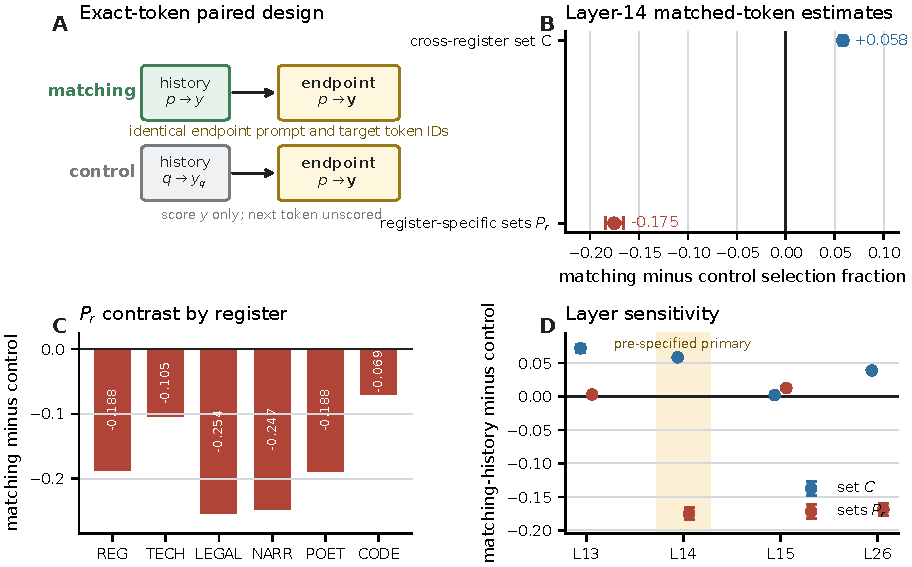
\includegraphics[width=\textwidth]{fig_clean_confirmation.pdf}
\caption{\textbf{Matched-token design and result.} (A) Both conditions
contain one prior turn and the same endpoint \(p\rightarrow y\); the matching
history repeats the full \(p\rightarrow y\) turn. (B) The two pre-specified
layer-14 contrasts with 95\% prompt-cluster bootstrap CIs. (C) Register-specific
\(P_r\) estimates are negative in all six registers. (D) Layer 26, a
trained copy of layer 14 in this checkpoint (Section~\ref{sec:layers}), is
directionally concordant; layers 13 and 15 do not reproduce the signed
decomposition. The shaded band marks the pre-specified primary layer. Values
are loaded from the archived result JSON by \texttt{make\_figs.py}.}
\label{fig:clean}
\end{figure*}

\subsection{Availability of the target reorganizes layer-14 routing at fixed token identity}

The generated study completed all 2,160 responses (360 paired turn-3
endpoints, 120 prompt clusters). Repeat-arm turn-3 copy fraction had median
0.961 against a varied-arm median of 0.000 (paired median difference 0.961;
85\% of repeat endpoints at or above 0.50), so the manipulation check passed.
At layer 14, repeat-minus-varied selection was \(+0.07966\) for \(C\)
(95\% CI \([+0.07396,+0.08531]\)) and \(-0.17675\) for \(P_r\)
(\([-0.18695,-0.16659]\)), negative in all six registers
(Table~\ref{tab:headline}). The pre-specified headline passed without expert
substitution.

The matched-token study, which removes token identity as an explanation,
completed all 720 rows; every one of the 360 pairs had identical target token
identities, and the median share of target eight-grams available in history
was 1.000 under matching and 0.000 under control (maximum control value
0.0925). Layer-14 matching-minus-control selection was \(+0.05828\) for \(C\)
(\([+0.05526,+0.06134]\)) and \(-0.17515\) for \(P_r\)
(\([-0.18406,-0.16604]\)), with all six register CIs below zero
(Figure~\ref{fig:clean}C). The redistribution is asymmetric: across the
generated, matched, and factorial estimates the normalized register-specific
decrease is two to four times the cross-register increase. Absolute values
show the same picture: under availability \(P_r\) selection falls from roughly
0.22 to 0.04, close to the uniform reference, while \(C\) rises from below
0.01 to between 0.07 and 0.09.

\subsection{The factorial attributes the reorganization to literal availability}

All 360 factorial quads retained identical scored target identities.
Availability produced the signed redistribution both without prompt
repetition (embed minus control) and with it (copy minus repeat;
Table~\ref{tab:factorial}). Repetition without availability was detectable
but small: 1.7\% of the copy-minus-control \(C\) contrast and 9.0\% of the
\(P_r\) contrast. Balanced main effects were \(+0.04923\) [0.04678, 0.05168]
(\(C\)) and \(-0.15571\) [\(-0.16952\), \(-0.14171\)] (\(P_r\)) for
availability, against \(+0.00797\) [0.00686, 0.00912] and \(-0.01899\)
[\(-0.02152\), \(-0.01656\)] for repetition; the nonzero interactions show
that repetition modestly amplifies the availability contrast.

\begin{table*}[t]
\small
\begin{tabularx}{\textwidth}{@{}lYYYYY@{}}
\toprule
\textbf{Readout} & \textbf{Avail., no rep.} & \textbf{Avail., rep.}
& \textbf{Rep., no avail.} & \textbf{Rep., avail.} & \textbf{Interaction} \\
\midrule
\(C\) & +0.04225 [0.04005, 0.04449] & +0.05621 [0.05320, 0.05924]
& +0.00099 [0.00045, 0.00167] & +0.01495 [0.01290, 0.01706]
& +0.01396 [0.01194, 0.01603] \\
\(P_r\) & \(-0.15242\) [\(-0.16542\), \(-0.13907\)] & \(-0.15901\) [\(-0.17376\), \(-0.14417\)]
& \(-0.01569\) [\(-0.01856\), \(-0.01295\)] & \(-0.02228\) [\(-0.02545\), \(-0.01919\)]
& \(-0.00659\) [\(-0.01006\), \(-0.00326\)] \\
\bottomrule
\end{tabularx}
\caption{\textbf{Layer-14 factorial contrasts.} Availability contrasts are
embed minus control and copy minus repeat; repetition contrasts are repeat
minus control and copy minus embed; interaction is copy minus embed minus
repeat plus control. Brackets are 95\% prompt-cluster bootstrap CIs.}
\label{tab:factorial}
\end{table*}

\subsection{The contrast survives matching on measured predictive certainty}

Availability lowered both predictive quantities substantially. Without
repetition, the availability contrast in mean predictive entropy was
\(-1.01240\) nats [\(-1.10240\), \(-0.92453\)] and in target surprisal
\(-0.75908\) [\(-0.81867\), \(-0.69965\)]; with repetition, \(-0.99228\)
[\(-1.08234\), \(-0.90344\)] and \(-0.78062\) [\(-0.84244\), \(-0.71914\)].
An earlier output-entropy-stratified analysis of the generated study (118
prompt clusters) was directionally consistent (\(C\) \(+0.06597\)
[0.05983, 0.07208]; \(P_r\) \(-0.14908\) [\(-0.16995\), \(-0.12880\)]) but
did not match on the two predictive measures. The
pre-declared 0.20-SD common-support analysis nevertheless retained 18,485 of
58,007 token pairs (31.9\%) in the no-repetition stratum and 18,877 (32.5\%)
in the repetition stratum, all 120 prompt clusters contributing to each. On
these token-identical, predictability-matched pairs both readouts kept their
pre-specified directions and excluded zero: without repetition, \(C\)
\(+0.03481\) [0.03217, 0.03747] and \(P_r\) \(-0.12315\)
[\(-0.13618\), \(-0.11040\)]; with repetition, \(C\) \(+0.04790\)
[0.04436, 0.05147] and \(P_r\) \(-0.13273\) [\(-0.14762\), \(-0.11844\)]. The
conclusion held at all three sensitivity calipers (retention 26.9--41.6\%
without repetition, 27.8--42.1\% with). Under the pre-specified rule this is
evidence beyond measured predictive entropy and target surprisal; whether
predictability contributes causally remains open.

\subsection{Layer specificity and cross-runtime stability}\label{sec:layers}

Layer 26 reproduced both matched-token directions (\(C\) \(+0.03879\)
\([+0.03644,+0.04115]\); \(P_r\) \(-0.16899\) \([-0.17759,-0.16033]\)) and
both generated-study directions (\(C\) \(+0.04027\) \([+0.03779,+0.04274]\);
\(P_r\) \(-0.16280\) \([-0.17296,-0.15286]\)). The captured neighbors did not:
in the matched study, layer 13 raised \(C\) (\(+0.07182\)
\([+0.06577,+0.07752]\)) with a small positive \(P_r\) contrast (\(+0.00293\)
\([+0.00119,+0.00465]\)), and layer 15 left \(C\) near zero (\(+0.00205\)
\([-0.00107,+0.00497]\)) with a positive \(P_r\) contrast (\(+0.01252\)
\([+0.00952,+0.01547]\)). These secondary intervals are descriptive and not
multiplicity-adjusted; the result is a pre-specified layer-14 signature with
layer-26 corroboration (Figure~\ref{fig:clean}D).

Layer 26 is not an independent layer. A pinned weight scan of this
checkpoint, released separately \cite{shorthill2026blocks}, finds that
decoder layers 20 to 31 are a trained copy of layers 8 to 19: at offset 12
the within-block cosines are 0.897 for the DeltaNet convolution and 0.522
for the key projection against \(-0.001\) outside the block, and 0.794 for
the router rows against a background of 0.264. Layer 26 is therefore layer
14's twin, and the layer-26 corroboration above is the same signature seen
through a copy, not corroboration from an unrelated layer. The signature's per-expert structure
mirrors accordingly: across the 256 experts, the top-8 membership gains
(availability minus control) at layer 14 correlate with those at layer 26
at \(+0.81\) on the Qwen3.5 confirmation bank (24 pairs) and \(+0.79\) on
the Qwen3.6 confirmation bank (12 pairs), against 0.00 to 0.06 for the two
non-twin control layers tested, 8 and 20; individual experts mirror
unevenly, consistent with twins that have diverged during training. Two
consequences follow: single-layer claims about layers 8 to 31 of this
checkpoint come in pairs, which motivates testing both corresponding layers,
as the follow-up in Section~\ref{sec:intervention} does. A separate paper on
repeated decoder blocks across Qwen-family checkpoints is in preparation;
the scan and its data are public.

Because the primary captures use a custom llama.cpp callback, a
condition-blind sample (six register-balanced paired clusters, 12 rows, 1,806
scored tokens per layer) was recomputed on an independent Hugging Face forward
pass (same pinned revision, BF16, eager attention, archived token identities)
under a manifest fixed before the run. Tokenwise correlation of the 256
pre-softmax router logits met the 0.99 threshold at all four layers (layer-14
median Pearson \(r=0.99969\)); mean top-8 overlap did not meet its 0.95
threshold (0.9451 at layer 14, that is 7.56 of eight experts; 0.9467, 0.9356,
and 0.9211 at layers 13, 15, and 26; the full layer-14 set matched on 62.2\%
of tokens, disagreement concentrating where the eighth
versus ninth logit margin was smallest). The pre-specified readouts were
nevertheless stable on this sample (\(C\) contrast 0.05854 in llama.cpp
against 0.05691 in Hugging Face; \(P_r\) \(-0.17499\) against \(-0.17400\)):
the group-level contrast is cross-runtime stable, while exact expert
membership is not implementation-invariant. A descriptive analysis of
selection across five relative-position bins of the target (in the artifact
release) shows the \(P_r\) separation present from the first bin and the
\(C\) separation building over the early bins.

\section{Mechanism, Replication, and Behavioral Load}\label{sec:mechanism}

The results above argue against token identity, prompt repetition, and
measured predictive certainty as sufficient explanations. Three follow-up
studies, each with endpoints or predictions declared before capture, ask what
carries the shift, whether it reproduces beyond the discovery checkpoint, and
whether it matters for generation. All three are pilot-scale and single-day.
The retrieval, mask and confirmation studies run on the Hugging Face stack
(BF16, eager attention); the intervention study reported here is a
corrected re-implementation on an MLX build of the successor checkpoint,
replacing the withdrawn version 1.0--1.1 result
(Section~\ref{sec:intervention}). Table~\ref{tab:mech} summarizes them.

\begin{table*}[!t]
\footnotesize
\begin{tabularx}{\textwidth}{@{}>{\raggedright\arraybackslash}p{0.25\textwidth}>{\raggedright\arraybackslash}p{0.27\textwidth}Y@{}}
\toprule
\textbf{Study (checkpoint; pairs or prompts)} & \textbf{Measure} & \textbf{Result} \\
\midrule
Attention retrieval (3.5-Base; 24 explanatory, 12 first-person pairs)
& attention mass on the prior copy, availability minus control
& explanatory \(+0.468\) [0.444, 0.491], 24 of 24 positive (mean under
availability 0.556); first-person \(+0.310\) [0.232, 0.390], 12 of 12
(mean 0.507) \\
& layer-14 top-8 Jaccard between conditions, position-matched
& 0.105 on the explanatory bank (range 0.06--0.23) \\
& expert-114 selection frequency, first-person bank
& lower under availability in 12 of 12, \(-0.178\) [\(-0.253\), \(-0.113\)] \\
\addlinespace
Attention-path mask (3.5-Base; 12 first-person pairs)
& span attention; layer-14 Jaccard to control; expert-114 frequency
& span mass 0.507 \(\rightarrow\) 0.000; Jaccard 0.268 \(\rightarrow\) 0.660
in 12 of 12; expert 114 recovers 0.109 \(\rightarrow\) 0.205 (control 0.287)
in 9 of 12 \\
\addlinespace
Cross-generation confirmation (3.6-Instruct; 12 fresh pairs)
& seven pre-specified experts, four predicted up and three down, sign
agreement in \(\ge 10\) of 12
& 7 of 7 confirmed, every CI excluding zero; largest increase \(+0.333\)
[0.282, 0.385], largest decrease \(-0.271\) [\(-0.375\), \(-0.157\)] \\
\addlinespace
Knockout at layer 14, dispatch-verified (3.6-Instruct, MLX; 12 prompts,
prior answer available)
& four confirmed increase-experts excluded before top-8 selection;
delivered occupancy 0.000
& 5 of 12 generations token-identical to baseline; overlap with the prior
answer 0.296 against 0.285 at baseline \\
Knockout at layers 14 and 26 (3.6-Instruct, MLX; 12 prompts)
& the same set excluded at both copies; delivered 0.000 at both
& 5 of 12 token-identical (the same five); overlap 0.295 \\
Forcing E118 at layer 14 (3.6-Instruct, MLX; 12 prompts \(\times\) 2
histories)
& \(+3\) gate bias before top-8; delivered 0.976 with, 0.531 without, the
prior answer
& with the prior answer: 1 of 12 token-identical, overlap 0.471; without
it: 0 of 12 token-identical, overlap with the absent target 0.229 against
0.286, and 0.000 with the unrelated answer that is present \\
Forcing E118 at layers 14 and 26 (3.6-Instruct, MLX; 12 prompts
\(\times\) 2 histories)
& delivered 0.985 and 0.952 with the prior answer
& with the prior answer: 1 of 12 token-identical, overlap 0.395; without
it: 1 of 12, overlap with the absent target 0.244 \\
\bottomrule
\end{tabularx}
\caption{\textbf{Mechanism, replication, and intervention summary.} 3.5-Base is
Qwen3.5-35B-A3B-Base; 3.6-Instruct is instruction-tuned Qwen3.6-35B-A3B.
Bootstrap CIs use 10,000 prompt-cluster resamples (seed 299792). Selection
frequency is the share of scored tokens at which the expert is among the eight
selected; Jaccard is the intersection over union of two top-8 sets; copy
fraction is defined in Section~\ref{sec:methods}. The intervention rows
replace the version 1.0--1.1 rows, which are withdrawn
(Section~\ref{sec:intervention}); MLX rows use 4-bit weights with 8-bit
router gates, and ``overlap'' is the eight-gram copy fraction against the
prompt's own greedy answer.}
\label{tab:mech}
\end{table*}

\subsection{Attention retrieval of the prior copy carries about half of the shift}

Pair construction follows the matched-token study: the availability condition
supplies a history containing the greedy answer \(y_i\) to prompt \(p_i\) and
re-asks \(p_i\); the control supplies a different same-register history; the
target \(y_i\) is teacher-forced in both. Documents use a raw
\texttt{Question:/Answer:} format, and neutral filler tokens after the shorter
history place target tokens at identical absolute positions in both
conditions, removing the position mismatch the factorial left uncontrolled.
Two banks were authored blind on the day of capture (24 explanatory-register
and 12 first-person-register prompts). The harness records, per target token,
attention mass on the history-answer span (averaged over heads and the ten
softmax-attention layers), dense router logits at layers 13, 14, 15, and 26,
and top-8 identities at all 40 layers.

Under availability roughly half of each target token's attention mass lands
on the prior copy, and the contrast is positive in every pair of both banks
(Table~\ref{tab:mech}). In the first-person bank the control history is also
first-person text, so the contrast isolates availability of the specific
target from register similarity. With positions matched, the layer-14 top-8
sets serving identical tokens overlap between conditions at a Jaccard index
(intersection over union) of 0.105: fewer than two of eight experts are
shared on average. One register-selective
expert makes the withdrawal concrete. Expert 114 at layer 14, characterized in
the companion report as a correlate of first-person composition
\cite{shorthill2026} and predicted there (2026-07-06) to disengage under
literal reuse, and since identified as one of several genre-selective
experts at that layer (an October 2026 control run with the same instrument
found larger, disjoint expert families for recipe and travel prose: 427 and
145 expert--layer positions across the model that separate the register
from its controls perfectly, against 90 for self-description), had factorial
selection frequencies of 0.0764 (control), 0.0723
(repetition alone), 0.0141 (availability alone), and 0.0102 (both); within
REG, 0.454 (control) against 0.056 (copy), with repetition at 0.426, and below
0.01 in every cell of the other five registers (token-pooled). The
first-person bank tested the pre-specified endpoint directly: lower under
availability in 12 of 12 pairs. Its register selectivity was re-measured at
BF16 on Qwen3.5-35B-A3B, as recorded in that run, in September 2026 (fire-to-control ratio 23 against
the compendium's 21.7); that re-measurement did not manipulate availability,
so the withdrawal result rests on the measurements reported here and on the
dated prediction in the companion record.

Masking that pathway moves routing back. On the first-person pairs an
additive \(-\infty\) mask removed attention from target positions onto the
history-answer span at the ten softmax-attention layers of the availability
condition, leaving the DeltaNet recurrence untouched, with predictions fixed
before the run. Span attention fell to 0.000; layer-14 agreement with the
control condition rose from Jaccard 0.268 to 0.660 in 12 of 12 pairs, and
expert-114 selection recovered toward its control level in 9 of 12. The
restoration is partial, consistent with history content also reaching the
router through the recurrent path. Exploratory router-input probes on the same
pairs (in the artifact release) are consistent with the mask result: adding
back each pair's availability shift along the recovered expert-114 router
direction at layer 14 (\(+0.8\) to \(+2.3\) logits) restored roughly forty
percent of the withdrawal (0.109 to 0.182 in 10 of 12 pairs), a
mean-replacement variant that destroys token-level variance in that direction
lowered selection instead (0.109 to 0.048), and the layer-14 shared-expert
gate was slightly higher under availability in 12 of 12 pairs (0.197 against
0.189). Zeroing the direction raised expert-114 selection (to 0.720 globally
and 0.668 at layer 14) because the zeroed component sits above typically
negative competing logits; that artifact bounds how such probes may be read.

\subsection{The set structure replicates across a model generation}

A 12-pair pilot on the instruction-tuned Qwen3.6-35B-A3B sibling, run in chat
format, showed the same retrieval contrast (12 of 12 positive, mean
\(+0.480\)) and a layer-14 turnover of comparable scale (Jaccard 0.384). Seven
candidate experts fixed from that pilot (four predicted to increase under
availability, three to decrease) were then tested on twelve fresh same-day
pairs under a pre-specified rule (sign agreement in at least ten of twelve per
expert, with an attention gate per pair): all twelve pairs passed the gate,
all seven candidates passed, and every bootstrap CI excludes zero
(Table~\ref{tab:mech}). The set structure of the main result therefore
reproduces across a model generation, with different expert indices in the
same roles.

\subsection{A corrected intervention: the confirmed set is not behaviorally inert}\label{sec:intervention}

Versions 1.0 and 1.1 of this paper reported a necessity test and a
sufficiency test at layer 14 on the instruction-tuned checkpoint: the four
confirmed increase-experts excluded from the top-8 (``selection verified
0.00''), and one of them forced in on 96.6\% of tokens, with every
generation token-identical to baseline in both directions. Those results
are withdrawn. The hooks replaced the dense logits that the Transformers
5.15.0 router returns but left the returned expert indices and weights
unchanged, and the block dispatches on the indices and weights; the
``verified'' occupancies were computed from the edited logits. A code
review found this on 2026-09-04, and a reproducer confirmed it on
2026-10-07: with the saved hooks the MoE output is bit-identical to
baseline, and a positive control that edits the dispatched indices changes
it.

The follow-up reported here re-implements both interventions so that
dispatch changes by construction. On an MLX build of Qwen3.6-35B-A3B
(4-bit weights, 8-bit router gates) the bias is added to the gate output
before the top-8 selection, and the expert indices actually passed to the
experts are monitored at layer 14 and at layer 26, its trained copy
(Section~\ref{sec:layers}); delivered-occupancy summaries, not per-step
index traces, are retained in the released artifacts. The design is the
one published: the same twelve explanatory prompts, \(y_i\) the greedy
answer to \(p_i\), the available history \([p_i \rightarrow y_i,\, p_i]\)
and the control history \([p_j \rightarrow y_j,\, p_i]\), greedy decoding
with a 200-token cap, one run per cell. Four predictions were written in
the run script before execution; they were not deposited in an
independently timestamped registry.

Delivered occupancy confirms the interventions: 0.000 for the excluded set
at every intervened layer, and 0.976 for the forced expert at layer 14 with
the prior answer available (0.985 and 0.952 at both copies), against 0.531
without it. The earlier 96.6\% and 52.0\% were, in retrospect, what
dispatch would have done had the edit reached it.

Behavior differs from the withdrawn result in both directions
(Table~\ref{tab:mech}). Excluding the four increase-experts at layer 14
changed the generated text in seven of twelve prompts, with first
divergence between tokens 18 and 64, without a detected average change in
eight-gram overlap with the available prior answer (0.296 against 0.285 at
baseline; per prompt the overlap moved both ways). Excluding the set at
both copies changed the same seven prompts and no others, so the prediction
that intervening at both corresponding layers would increase the number of
divergent outputs failed. Forcing E118 at layer 14 changed eleven of twelve
outputs and raised overlap with the available prior answer from 0.285 to
0.471 (0.395 at both copies). In the control history, where the target
answer is absent and an unrelated answer is present, forcing changed twelve of twelve outputs at layer 14 alone and eleven of
twelve when applied at both corresponding layers, produced no overlap with the unrelated present answer (0.000), and
left overlap with the absent target at 0.229 (0.244 at both copies) against
0.286 at the control baseline; the same prompt regenerates similar wording
without the answer in context, so this is not evidence of retrieval. The
prediction that forcing would leave reuse unchanged was wrong.

The replacement for the withdrawn sentence is therefore direct: in this
follow-up, excluding the four increase-experts changed generated text in
seven of twelve prompts without a detected average reduction in reference
overlap, and forcing E118 increased overlap with an available prior answer
and changed eleven of twelve outputs. The layer-14 set carries a measurable
behavioral load where we intervened. The follow-up is a corrected
implementation, not a matched replication: it used the successor checkpoint
at reduced precision, greedy decoding, one run per cell and twelve prompts,
and its baseline overlap (0.285) is lower than the August report's (0.426).
A checkpoint- and precision-matched rerun on Qwen3.5-35B-A3B-Base at BF16,
and the same interventions on other models, including other
depth-duplicated checkpoints, would be useful; neither has been run.

\section{Discussion}\label{sec:discussion}

\paragraph{The confound.}
The pattern that emerges is uniform across designs: holding the endpoint fixed
and varying only whether the target text is already in context moves
layer-14 routing by an amount comparable to the entire register-specific
selection signal (\(P_r\) falls from about 0.22 to about 0.04, near the
uniform reference), in a direction fixed before capture, on two model
generations, and on token positions matched for predictive certainty. This is
a multi-turn evaluation contamination result on the measurement side.
Repeated or near-repeated multi-turn probes place later target strings in the
preceding context; once they do, any evaluation that reads internal state
(routing statistics, expert-selection profiles, or classifiers and probes
built on them, of the kind used for specialization benchmarks
\cite{wang2026dbes}, reasoning-state signals \cite{chen2026},
context-faithfulness experts \cite{bai2025}, and safety telemetry
\cite{lv2026}) partly measures whether the text was available for reuse,
with a smaller contribution from prompt repetition and its interaction, in
addition to the capability nominally under evaluation. The corrected
interventions bound the claim differently from versions 1.0 and 1.1:
excluding the confirmed set changes generated text in most prompts but does
not reduce reuse of the available answer on average, so we do not claim
that availability shifts output-level scores, and we no longer claim that
the set is inert.
For MoE interpretability, \(n\)-gram availability of the target, exact
prior-turn matching, and predictive certainty are therefore design covariates
to report or control. This is a recommendation from one model family observed
on two of its generations; a cross-family standard would require the design
on unrelated MoE lineages.

\paragraph{Readout versus load.}
The second implication concerns how routing signatures are read, and it is
the paragraph that changed most between versions. The Qwen3.6 set passed a
pre-specified confirmation with every interval excluding zero; versions 1.0
and 1.1 then reported it inert under knockout and forcing, and drew the
lesson that replicated observational signatures license neither necessity
nor sufficiency claims. The lesson stands, for a sharper reason: the
interventions that seemed to show inertness had not reached dispatch, and
when they did, the set turned out to carry a measurable load, with text
changing in most prompts under exclusion and reuse rising under forcing. A
replicated signature identifies a readout of a condition; what its experts
do is a separate question, and the answer depends on the intervention being
implemented at the point where routing is decided. This accords with the
pre-registered causal test in which apparent expert modularity largely
dissolved \cite{salomone2026} and with accounts that locate routing
structure in representation geometry rather than expert function
\cite{wang2026myth}. The discovery-stage labels for our sets described
selection contrasts; functional readings require evidence beyond selection
statistics, and require checking that the intervention code changes what
the model computes.

\paragraph{Scope.}
The between-register spread of the matched \(P_r\) contrast (CODE
\(-0.06935\) \([-0.08267,-0.05664]\) to LEGAL \(-0.25370\)
\([-0.27548,-0.23240]\)) was not a pre-specified test; each register uses a
different set and different control selection (0.087 for CODE against 0.319
for LEGAL), so the spread does not show that legal text is intrinsically more
sensitive. The source response in the matching history was produced by the
same model, but the design does not compare self-generated with externally
supplied identical text; the claim concerns literal availability, of which
same-model source was one feature. A pre-registered companion study on dense
Qwen3-8B, reported separately, finds the same manipulation lowering a
residual-stream vocabulary readout, which ties the availability variable,
through a different instrument, to a checkpoint with no routing at all. None
of these routing measurements bears on model experience or on the accuracy of
elicited self-report.

\section{Limitations}\label{sec:limitations}

\begin{enumerate}[leftmargin=1.4em,itemsep=2pt]
\item \textbf{Evidential standards differ across components.} The
pre-specified bank battery ran on Qwen3.5-35B-A3B-Base with one
machine-generated 120-prompt bank; the holdout and unrelated MoE families are
untested at that standard. The Qwen3.6 evidence is a same-day pre-specified
confirmation at 12-pair scale in chat format, and the mechanism study uses 36
pairs, one day, one stack, and a raw-text format rather than the dialogue
template. The corrected intervention follow-up uses the successor checkpoint
on an MLX build at 4-bit weight precision with 8-bit router gates, twelve
prompts, greedy decoding and one run per cell; it is a corrected
implementation of the withdrawn result, not a checkpoint- and
precision-matched replication of it.
\item \textbf{The factorial does not equalize every history property.}
\(y'\) is a different-seed answer and \(y_q\) answers a different prompt, so
prior-answer semantics, lengths, and absolute target positions vary across
cells (the mechanism study matches positions; the factorial does not).
Repetition and the interaction are small but nonzero. The supported claim is
availability dominance in this construction.
\item \textbf{Teacher forcing changes the task.} The matched and factorial
studies score routing on a fixed target; the generated study supplies the
complementary free-generation comparison, but the two estimands differ.
\item \textbf{Predictability is not excluded as a mechanism.} Matching on
post-treatment entropy and surprisal retains the contrast but does not
estimate mediation or rule out a causal role for predictability.
\item \textbf{Sets are model-relative and membership is
implementation-sensitive.} \(C\) and \(P_r\) were selected on the same
checkpoint and confirmed on new prompts, which guards against post hoc
substitution but does not establish portable identities or functions. Only
four layers were captured, the signed decomposition was absent at both
captured neighbors, and the independent stack reproduced logits and contrasts
closely while missing the 0.95 top-8 overlap threshold; the main CIs quantify
prompt sampling only. Layers 8 to 31 of this checkpoint come in twin pairs
at offset 12 (Section~\ref{sec:layers}), so layer 26 is not an independent
corroborating layer.
\item \textbf{Interventions sever or force one path at one or two layers.}
The attention mask leaves the recurrent path untouched and restores routing
partially; the corrected knockout and forcing tests show a behavioral load
at layer 14 and its copy without locating the rest of it, retain
delivered-occupancy summaries rather than per-step expert-index traces, and
recorded their predictions in the run script without an independently
timestamped snapshot; no mediation quantity is estimated, and the
router-direction probes are exploratory.
\end{enumerate}

\section{Conclusion}\label{sec:conclusion}

Whether the text a mixture-of-experts model is processing is already
available verbatim in its context is a routing-relevant variable in its own
right. In Qwen3.5-35B-A3B-Base it reorganizes layer-14 expert selection in a
direction fixed before capture, independently of token identity, prompt
repetition, and measured predictive certainty; the shift is carried in
substantial part by attention retrieval of the prior copy; its set structure
reproduces on instruction-tuned Qwen3.6-35B-A3B under pre-specified
predictions; and, in a corrected-implementation follow-up, excluding the
confirmed set changes generated text in most prompts without a detected
average reduction in reuse of the available answer, while forcing one of its experts
increases reuse. Two consequences follow for practice. Multi-turn probes
that place later target text in earlier context contaminate routing-based and
related internal-state measurements with availability, so such evaluations
partly measure reusability in addition to the capability they name, and
availability should be treated as a design covariate. And a routing
signature that replicates under pre-specified rules is evidence of a reliable
readout; a causal role is a separate claim that requires an intervention
implemented where routing is decided. Where we first intervened, the code
never reached that point; where it did, the set did something measurable.
The signature is real and replicable, and its experts carry a load that the
readout alone could not reveal.

\section*{Ethics Statement}

No human subjects or private data were involved. Some REG prompts ask the
model for first-person descriptions; all such text is treated as behavioral
output, and the study measures routing and exact string recurrence only.
Reporting the excluded malformed-marker pilot and the exact-token gates is
part of the risk control against drawing conclusions from a mis-specified
instrument.

\section*{Author Note and AI Collaboration Statement}

The data-collection and analysis pipeline and the manuscript were prepared
with the assistance of Claude Fable~5 (Anthropic): the model wrote and
operated capture and analysis tooling, executed data-collection runs under the
author's direction, and assisted with drafting, critique, and organization.
The human author selected the claims, fixed the experimental decisions,
directed the captures, reviewed the reported values against the result files,
and takes responsibility for the manuscript. The error in the version
1.0--1.1 intervention hooks was found by a code review carried out with a
second language model (OpenAI Codex) on 2026-09-04 and reproduced by Claude
Fable~5.1 on 2026-10-07, which also ran the corrected follow-up. An independent review with OpenAI
Codex checked the revised claims and reported values against the source
artifacts before this version was deposited. No language model is an
author.
The prompt bank was generated by \texttt{anthropic/claude-5-fable-20260609}
through OpenRouter and was split and validated mechanically without
routing-based selection.

\section*{Funding and Competing Interests}

This work received no external funding. The author declares no competing
interests.

\section*{Data and Artifact Availability}

The public artifact release is at
\url{https://huggingface.co/datasets/ec75hash/qwen35-exact-turn-routing/tree/v1.3.1}:
raw router archives, exact token surfaces, compact results, pre-specified
analysis specifications and capture code, the publication re-analysis, the
reference-stack logits and metrics, paper source, and release-wide SHA-256
digests. The generated-study and matched-study specification digests begin
\texttt{7aa33f9ad3328891} and \texttt{6c6501cc618ccffe}; the raw archive
digests begin \texttt{0b1b31477db97b30} and \texttt{8fa63e2ea31bcfb3}. The
factorial and predictability extension is under
\texttt{extension/20260809T193509Z-f02} (1,440-row JSONL SHA-256 beginning
\texttt{3732288a13f77a5e}); the mechanism-study arrays, intervention captures,
blind banks, pre-specified Qwen3.6 candidate list, and capture harnesses are
under \texttt{extension/20260812-mechanism-crossgen/}; the data, script, paper and extension files are covered by
the release-wide \texttt{SHA256SUMS} manifest. Specifications were fixed and
hash-committed locally before capture and enforced by the run pipeline; they
were not deposited in a public timestamped registry before data collection.
The 60-prompt holdout is public but unused. Model weights are not
redistributed; the release records the exact Hugging Face revision, GGUF hash,
and llama.cpp commit. Version 1.2 adds the corrected intervention follow-up
under \texttt{extension/\allowbreak 20261007-dispatch-verified-interventions/} (dataset
v1.3.1): the run script with its pre-run predictions, generated token
identities, delivered-occupancy summaries, overlap measurements, and the
result record with its dated correction. Dataset versions map to paper
versions as follows: dataset v1.1 to paper v0.9.1, dataset v1.2 to paper
v1.0 through v1.1, dataset v1.3 and v1.3.1 to paper v1.2; earlier labels are
preserved. The August intervention captures in
\texttt{extension/20260812-mechanism-crossgen/} record edited logits, not
executed routing, and are retained as the record of the withdrawn result.
The repeated-block scan cited in Section~\ref{sec:layers} is archived as
\cite{shorthill2026blocks}. Earlier exploratory batteries remain in the
companion technical report \cite{shorthill2026}, a program record that was
files-restricted from 2026-09-03 to 2026-10-21 and is open again with a
status note; several of its readings were later narrowed, and it should be
read as a lab record rather than as current claims.

\begin{thebibliography}{20}
\footnotesize

\bibitem[Antoine et al.(2025)]{antoine2025}
Elie Antoine, Frederic Bechet, and Philippe Langlais. 2025. Part-of-speech
sensitivity of routers in mixture of experts models. In \emph{COLING}, pages
6467--6474.

\bibitem[Arnold et al.(2024)]{arnold2024}
Stefan Arnold, Marian Fietta, and Dilara Yesilbas. 2024. Routing in
sparsely-gated language models responds to context. In \emph{BlackboxNLP}, pages
15--22. DOI: \href{https://doi.org/10.18653/v1/2024.blackboxnlp-1.2}{10.18653/v1/2024.blackboxnlp-1.2}.

\bibitem[Bai et al.(2025)]{bai2025}
Jun Bai, Minghao Tong, Yang Liu, Zixia Jia, and Zilong Zheng. 2025.
Understanding and leveraging the expert specialization of context faithfulness
in mixture-of-experts LLMs. In \emph{EMNLP}, pages 21927--21942.

\bibitem[Chen et al.(2026)]{chen2026}
Kang Chen, Minshen Yu, Junjie Nian, Yaoning Wang, Yixin Cao, and Yugang Jiang.
2026. Does the same token mean the same state? MoE routing as signal for
reasoning control. \href{https://arxiv.org/abs/2606.22798}{arXiv:2606.22798}.

\bibitem[Fedus et al.(2022)]{fedus2022}
William Fedus, Barret Zoph, and Noam Shazeer. 2022. Switch Transformers:
Scaling to trillion parameter models with simple and efficient sparsity.
\emph{JMLR}, 23(120):1--39.

\bibitem[Holtzman et al.(2020)]{holtzman2020}
Ari Holtzman, Jan Buys, Li Du, Maxwell Forbes, and Yejin Choi. 2020. The
curious case of neural text degeneration. In \emph{ICLR}.

\bibitem[Lv et al.(2026)]{lv2026}
Bo Lv, Zhiheng Xu, KeDong Xiu, Ruyi Ding, Tianhang Zheng, Zhibo Wang, and Kui
Ren. 2026. RouteScan: A non-intrusive approach to auditing MoE LLMs safety via
expert routing telemetry. \href{https://arxiv.org/abs/2605.24817}{arXiv:2605.24817}.

\bibitem[Olson et al.(2025)]{olson2025}
Matthew Lyle Olson, Neale Ratzlaff, Musashi Hinck, Man Luo, Sungduk Yu, Chendi
Xue, and Vasudev Lal. 2025. Probing semantic routing in large mixture-of-expert
models. In \emph{Findings of EMNLP}, pages 18263--18278.

\bibitem[Olsson et al.(2022)]{olsson2022}
Catherine Olsson, Nelson Elhage, Neel Nanda, et al. 2022. In-context learning
and induction heads. \emph{Transformer Circuits Thread}. \href{https://arxiv.org/abs/2209.11895}{arXiv:2209.11895}.

\bibitem[Qwen Team(2026)]{qwen2026}
Qwen Team. 2026. Qwen3.5: Towards native multimodal agents.
\url{https://qwen.ai/blog?id=qwen3.5}.

\bibitem[Salomone et al.(2026)]{salomone2026}
Tony Salomone, Deep Gandhi, and Ali Asaria. 2026. How modular is a frontier
mixture-of-experts? A pre-registered causal test in which apparent expert
modularity mostly dissolves. \href{https://arxiv.org/abs/2606.25092}{arXiv:2606.25092}.

\bibitem[Shazeer et al.(2017)]{shazeer2017}
Noam Shazeer, Azalia Mirhoseini, Krzysztof Maziarz, Andy Davis, Quoc Le,
Geoffrey Hinton, and Jeff Dean. 2017. Outrageously large neural networks: The
sparsely-gated mixture-of-experts layer. In \emph{ICLR}.

\bibitem[Shorthill(2026a)]{shorthill2026}
Jeffrey William Shorthill. 2026a. Composition-sensitive register readouts in
mixture-of-experts routing (program compendium). Zenodo.
DOI: \href{https://doi.org/10.5281/zenodo.20709736}{10.5281/zenodo.20709736}.

\bibitem[Shorthill(2026b)]{shorthill2026blocks}
Jeffrey William Shorthill. 2026b. Repeated blocks in Qwen-family
checkpoints: pinned weight scans, v0.1.2. Zenodo.
DOI: \href{https://doi.org/10.5281/zenodo.23546828}{10.5281/zenodo.23546828}.

\bibitem[Wang(2026)]{wang2026rep}
Han-yu Wang. 2026. When more becomes less: Position-dependent repetition
effects in language models. \href{https://arxiv.org/abs/2608.04021}{arXiv:2608.04021}.

\bibitem[Wang et al.(2026a)]{wang2026dbes}
Jing Wang, Hongxuan Lu, Jazze Young, Shu Wang, and Zhimin Xin. 2026. DBES: A
systematic benchmark and metric suite for evaluating expert specialization in
large-scale MoEs. \href{https://arxiv.org/abs/2605.18498}{arXiv:2605.18498}.

\bibitem[Wang et al.(2026b)]{wang2026myth}
Xi Wang, Soufiane Hayou, and Eric Nalisnick. 2026. The myth of expert
specialization in MoEs: Why routing reflects geometry, not necessarily domain
expertise. \href{https://arxiv.org/abs/2604.09780}{arXiv:2604.09780}.

\bibitem[Wang et al.(2026c)]{wang2026}
Yan Wang, Yitao Xu, Nanhan Shen, Jinyan Su, Jimin Huang, and Zining Zhu. 2026.
The illusion of specialization: Unveiling the domain-invariant standing
committee in mixture-of-experts models. In \emph{ACL}, pages 14601--14618.

\bibitem[Welleck et al.(2020)]{welleck2020}
Sean Welleck, Ilia Kulikov, Stephen Roller, Emily Dinan, Kyunghyun Cho, and
Jason Weston. 2020. Neural text generation with unlikelihood training. In
\emph{ICLR}.

\bibitem[Ye et al.(2026)]{ye2026}
Charles Ye, Bo Yuan, and Lee Sharkey. 2026. Polysemantic experts, monosemantic
paths: Routing as control in MoEs. \href{https://arxiv.org/abs/2604.17837}{arXiv:2604.17837}.

\bibitem[Yoon et al.(2026)]{yoon2026}
Youngsik Yoon, Siwei Wang, Wei Chen, and Jungseul Ok. 2026. When are experts
misrouted? Counterfactual routing analysis in mixture-of-experts language
models. \href{https://arxiv.org/abs/2605.07260}{arXiv:2605.07260}.

\end{thebibliography}

\end{document}
